%iffalse
\let\negmedspace\undefined
\let\negthickspace\undefined
\documentclass[journal,12pt,onecolumn]{IEEEtran}
\usepackage{cite}
\usepackage{amsmath,amssymb,amsfonts,amsthm}
\usepackage{algorithmic}
\usepackage{graphicx}
\usepackage{textcomp}
\usepackage{xcolor}
\usepackage{txfonts}
\usepackage{listings}
\usepackage{enumitem}
\usepackage{enumitem,multicol}
\usepackage{mathtools}
\usepackage{gensymb}
\usepackage{comment}
\usepackage[breaklinks=true]{hyperref}
\usepackage{tkz-euclide} 
\usepackage{listings}
\usepackage{gvv}                                        
%\def\inputGnumericTable{}                                 
\usepackage[latin1]{inputenc}                                
\usepackage{color}                                            
\usepackage{array}                                            
\usepackage{longtable}                                       
\usepackage{calc}                                             
\usepackage{multirow}                                         
\usepackage{hhline}                                           
\usepackage{ifthen}                                           
\usepackage{lscape}
\usepackage{tabularx}
\usepackage{array}
\usepackage{float}
\usepackage[american,siunitx]{circuitikz}
\usetikzlibrary{arrows,shapes,calc,positioning}
\usepackage{pgfplots}


\newtheorem{theorem}{Theorem}[section]
\newtheorem{problem}{Problem}
\newtheorem{proposition}{Proposition}[section]
\newtheorem{lemma}{Lemma}[section]
\newtheorem{corollary}[theorem]{Corollary}
\newtheorem{example}{Example}[section]
\newtheorem{definition}[problem]{Definition}
\newcommand{\BEQA}{\begin{eqnarray}}
\newcommand{\EEQA}{\end{eqnarray}}
\newcommand{\define}{\stackrel{\triangle}{=}}
\theoremstyle{remark}
\newtheorem{rem}{Remark}

% Marks the beginning of the document
\begin{document}
\bibliographystyle{IEEEtran}
\vspace{3cm}

\title{XE-2016}
\author{EE24Btech11022 - Eshan Sharma}
\maketitle

\renewcommand{\thefigure}{\theenumi}
\renewcommand{\thetable}{\theenumi}



\begin{enumerate}
\item The flow field shown over a bluff body has considerably curved streamlines. A student measures pressures at points $A$, $B$, $C$, and $D$ and denotes them as $P_A$, $P_B$, $P_C$, and $P_D$ respectively. State which one of the following statements is true. The arrow indicates the freestream flow direction.\\

\begin{center}
	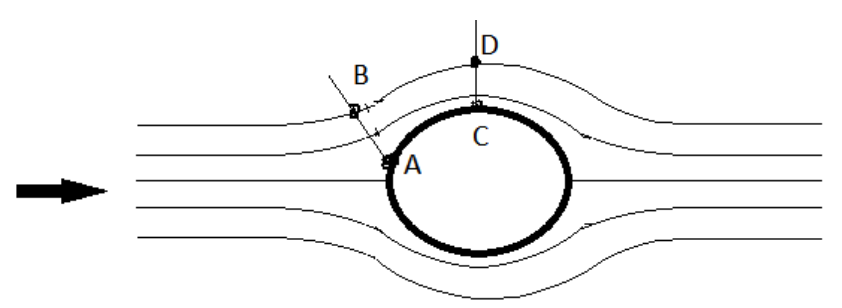
\includegraphics[width=0.6\textwidth]{figs/27.png}
\end{center}

\begin{enumerate}
	\item $P_A = P_B$ and $P_C > P_D$
	\item $P_A > P_B$ and $P_C > P_D$
	\item $P_A = P_B$ and $P_C < P_D$
	\item $P_A > P_B$ and $P_C < P_D$\\
\end{enumerate}

\item A 2-D incompressible flow is defined by its velocity components in m/s as $u = -\frac{c y}{x^2 + y^2}$ and $v = \frac{cx}{x^2 + y^2}$. If the value of the constant $c$ is equal to 0.1 m\(^3\), the numerical value of vorticity at the point $x = 1$ m and $y = 2$ m is \_\_\_\_\_ s\(^{-1}\).\\

\item Two flow configurations are shown below for flow of incompressible, viscous flow. The inlet velocity for the diverging nozzle (Fig (i)) and free-stream velocity for flow past the bluff body (Fig (ii)) is constant. Points $A$ and $B$ are separation points and flow is laminar. The relation regarding velocity gradients at point $A$ and $B$ is ($y$ is the direction normal to the surface at the point of separation).\\

\begin{center}
	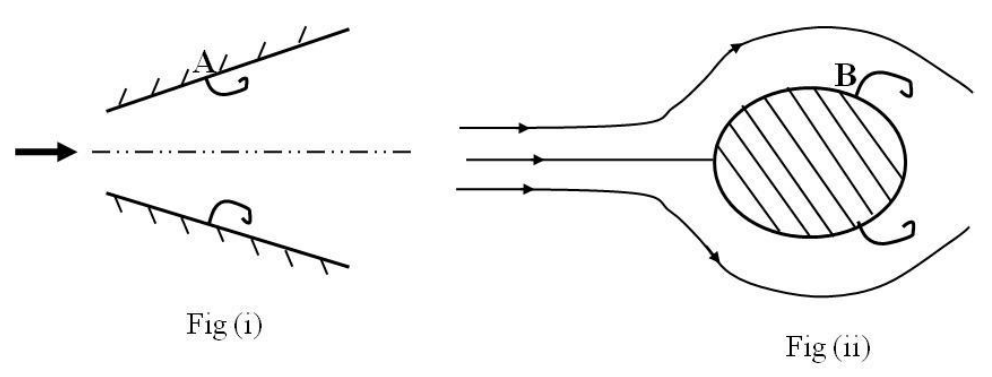
\includegraphics[width=0.8\textwidth]{figs/29.png}
\end{center}

\begin{enumerate}
\begin{multicols}{4}
	\item $\frac{\partial u}{\partial y}\bigg|_A = \frac{\partial u}{\partial y}\bigg|_B$
	\item $\frac{\partial u}{\partial y}\bigg|_A > \frac{\partial u}{\partial y}\bigg|_B$
	\item $\frac{\partial u}{\partial y}\bigg|_A < \frac{\partial u}{\partial y}\bigg|_B$
	\item $\frac{\partial^{2} u}{\partial y^{2}}\bigg|_A = \frac{\partial^{2} u}{\partial y^{2}}\bigg|_B$
\end{multicols}
\end{enumerate}

\item Consider a fully developed, steady, incompressible, 2-D, viscous channel flow with uniform suction and blowing velocity $v_0$ as shown in the figure below. The centerline velocity of the channel is 10 m/s along the $x$-direction. If the value of $v_0$ at both the walls is 1 m/s, the value of the $y$-component of velocity inside the flow field is \_\_\_\_\_ m/s.\\

\begin{figure}[!ht]
	\centering
	\resizebox{0.6\textwidth}{!}{%
		\begin{circuitikz}
			\tikzstyle{every node}=[font=\LARGE]
			\draw [->, >=Stealth] (8,10) .. controls (8,9.5) and (8,9.25) .. (8,10) ;
			
			\draw (7.25,14.25) to[short] (17.75,14.25);
			\draw (7.25,10) to[short] (18,10);
			\draw [->, >=Stealth] (8,14.25) -- (8,14.75);
			\draw [->, >=Stealth] (8.75,14.25) -- (8.75,14.75);
			\draw [->, >=Stealth] (9.5,14.25) -- (9.5,14.75);
			\draw [->, >=Stealth] (10.25,14.25) -- (10.25,14.75);
			\draw [->, >=Stealth] (11,14.25) -- (11,14.75);
			\draw [->, >=Stealth] (11.75,14.25) -- (11.75,14.75);
			\draw [->, >=Stealth] (12.5,14.25) -- (12.5,14.75);
			\draw [->, >=Stealth] (13.25,14.25) -- (13.25,14.75);
			\draw [->, >=Stealth] (14,14.25) -- (14,14.75);
			\draw [->, >=Stealth] (14.75,14.25) -- (14.75,14.75);
			\draw [->, >=Stealth] (15.5,14.25) -- (15.5,14.75);
			\draw [->, >=Stealth] (16.25,14.25) -- (16.25,14.75);
			\draw [->, >=Stealth] (17,14.25) -- (17,14.75);
			\draw [dashed] (7.25,12.25) -- (17.75,12.25);
			\draw [->, >=Stealth] (7.25,12.25) -- (7.25,13.5);
			\draw [->, >=Stealth] (7.25,12.25) -- (8.5,12.25);
			\node [font=\LARGE] at (8.25,11.75) {x};
			\node [font=\LARGE] at (6.75,13.5) {y};
			\draw [line width=2pt, ->, >=Stealth] (5,12.25) -- (6.25,12.25);
			\draw [line width=0.6pt, ->, >=Stealth] (8.75,9.5) -- (8.75,10);
			\draw [line width=0.6pt, ->, >=Stealth] (9.5,9.5) -- (9.5,10);
			\draw [line width=0.6pt, ->, >=Stealth] (10.25,9.5) -- (10.25,10);
			\draw [line width=0.6pt, ->, >=Stealth] (11,9.5) -- (11,10);
			\draw [line width=0.6pt, ->, >=Stealth] (11.75,9.5) -- (11.75,10);
			\draw [line width=0.6pt, ->, >=Stealth] (12.5,9.5) -- (12.5,10);
			\draw [line width=0.6pt, ->, >=Stealth] (13.25,9.5) -- (13.25,10);
			\draw [line width=0.6pt, ->, >=Stealth] (14,9.5) -- (14,10);
			\draw [line width=0.6pt, ->, >=Stealth] (14.75,9.5) -- (14.75,10);
			\draw [line width=0.6pt, ->, >=Stealth] (15.5,9.5) -- (15.5,10);
			\draw [line width=0.6pt, ->, >=Stealth] (16.25,9.5) -- (16.25,10);
			\draw [line width=0.6pt, ->, >=Stealth] (17,9.5) -- (17,10);
			\node [font=\LARGE] at (12.25,15.5) {$v_0$};
			\node [font=\LARGE] at (12.5,8.75) {$v_0$};
		\end{circuitikz}
	}%
	
	\label{x}
\end{figure}


\item Exhaust from a kitchen goes into the atmosphere through a tapered chimney as shown. The area of cross-section of a chimney at location-1 is twice of that at location-2. The flow rate is assumed to be steady with constant exhaust density of 1 kg/m$^3$ and acceleration due to gravity, $g = 9.8$ m/s$^2$. If the steady uniform exhaust velocity at location-1 is $U = 1$ m/s, the pressure drop across the chimney is \_\_\_\_ Pa.\\

\begin{figure}[!ht]
	\centering
	\resizebox{0.6\textwidth}{!}{%
		\begin{circuitikz}
			\tikzstyle{every node}=[font=\LARGE]
			\draw [ line width=0.9pt](5.75,11.25) to[short] (8.75,11.25);
			\draw [ line width=0.9pt](8.75,11.25) to[short] (11.5,14);
			\draw [ line width=0.9pt](13.5,14) to[short] (16.25,11.25);
			\draw [ line width=0.9pt](16.25,11.25) to[short] (19.5,11.25);
			\draw [line width=0.9pt, dashed] (8.75,11.25) -- (16.25,11.25);
			\draw [line width=0.9pt, ->, >=Stealth] (12.5,12.25) -- (12.5,13.25);
			\draw [line width=0.9pt, dashed] (11.5,14) -- (13.5,14);
			\draw [line width=0.9pt, short] (15.25,14) -- (17.75,14);
			\draw [line width=0.9pt, <->, >=Stealth] (16.75,14) -- (16.75,11.25);
			\node [font=\LARGE] at (17.5,12.75) {150 mm};
			\node [font=\LARGE] at (12.5,11) {1};
			\node [font=\LARGE] at (12.5,14) {2};
			\draw [ line width=0.9pt ] (12.5,14) circle (0.5cm);
			\draw [ line width=0.9pt ] (12.5,11) circle (0.5cm);
		\end{circuitikz}
	}%
	
	\label{fig:my_label}
\end{figure}

\item A jet of diameter 20 mm and velocity 6 m/s coming out of a water-tank standing on a frictionless cart hits a vane and gets deflected at an angle of 45\degree\ as shown in the figure below. The density of water is 1000 kg/m$^3$. Neglect all minor and viscous losses. If the cart remains stationary, the magnitude of tension in the supporting string connected to the wall is \_\_\_\_ N.\\

\begin{figure}[!ht]
	\centering
	\resizebox{0.6\textwidth}{!}{%
		\begin{circuitikz}
			\tikzstyle{every node}=[font=\normalsize]
			\draw [line width=1pt, short] (7.25,17.25) -- (7.25,10.5);
			\draw [line width=1pt, short] (7.25,10.5) -- (12.5,10.5);
			\draw [line width=1pt, short] (12.5,10.5) -- (12.5,12);
			\draw [line width=1pt, short] (12.5,13) -- (12.5,17.25);
			\draw [line width=1pt, short] (12.5,13) -- (14.25,13);
			\draw [line width=1pt, short] (12.5,12) -- (14.25,12);
			\draw [line width=1pt, dashed] (7.25,16.5) -- (12.5,16.5);
			\draw [line width=1pt, <->, >=Stealth] (7.25,14.75) -- (12.5,14.75);
			\draw [line width=1pt, short] (9.75,16.5) -- (9.5,15.75);
			\draw [line width=1pt, short] (9.75,16.5) -- (10,15.75);
			\draw [line width=1pt, short] (9.5,15.75) -- (10,15.75);
			\draw [ line width=1pt ] (8.75,10) circle (0.5cm);
			\draw [ line width=1pt ] (6.75,9.5) rectangle (23,9.25);
			\draw [ line width=1pt ] (10.75,10) circle (0.5cm);
			\draw [ line width=1pt ] (22.75,12.75) rectangle (23,9.5);
			\draw [ line width=1pt ] (12.5,11) rectangle (18,10.75);
			\draw [ line width=1pt ] (17.25,12) rectangle (17.5,11);
			\draw [ line width=1pt ] (16.75,12) rectangle (17.25,11.75);
			\draw [ line width=1pt ] (17.25,12) -- (17.5,12) -- (19.5,14.5) -- (19.25,14.5) -- cycle;
			\draw [line width=1.8pt, short] (18,11) -- (22.75,11);
			\draw [line width=1.8pt, short] (6.75,9.5) -- (23,9.5);
			\draw [line width=1.8pt, short] (22.75,12.75) -- (22.75,9.5);
			\draw [line width=1.8pt, short] (14,12.75) -- (14,12);
			\draw [line width=1.8pt, short] (14,12.75) -- (16.75,12.75);
			\draw [line width=1.8pt, short] (14,12) -- (17.25,12);
			\draw [line width=1.8pt, short] (16.75,12.75) -- (19.5,16.25);
			\draw [line width=1.8pt, short] (19.5,16.25) -- (20.5,16.25);
			\draw [line width=1.8pt, short] (20.5,16.25) -- (17.25,12);
			\draw [line width=1.1pt, ->, >=Stealth] (20,16.25) -- (20.75,17.25);
			\draw [line width=1.1pt, ->, >=Stealth] (11.75,12.5) -- (13,12.5);
			\draw [line width=1.1pt, short] (19.25,14.5) -- (20.75,14.5);
			\draw [line width=1.1pt, ->, >=Stealth] (20.25,14.5) .. controls (20.25,15) and (20.25,15) .. (20,15.5) ;
			\node [font=\LARGE] at (20,11.5) {string};
			\node [font=\Large] at (19,16.75) {$6 m/s$};
			\node [font=\Large] at (21,15) {$45\circ$};
			\node [font=\LARGE] at (9.5,14) {$D = 3 m$};
			\node [font=\normalsize] at (13.5,13.25) {$D_0 = 20 mm$};
		\end{circuitikz}
	}%
	
	\label{fig:my_label}
\end{figure}


\item A block is floating at the oil-water interface as shown. The density of oil is two-thirds that of water. Given that the density of the block is 800 kg/m$^3$ and that of water is 1000 kg/m$^3$, the fraction of the total height of block in oil is \_\_\_\_.\\

\begin{figure}[!ht]
	\centering
	\resizebox{0.3\textwidth}{!}{%
		\begin{circuitikz}
			\tikzstyle{every node}=[font=\LARGE]
			%\draw[fill={rgb,255:red,255; green,255; blue,255}] (7,16.75) rectangle (15.75,8);
			\draw [ line width=0.9pt ] (8,15.25) rectangle (14.75,9);
			\draw [line width=0.9pt, short] (8,15.25) -- (8,15.75);
			\draw [line width=0.9pt, short] (14.75,15.25) -- (14.75,15.75);
			\draw [ line width=0.9pt ] (10,12.75) rectangle (12.75,11);
			\node [font=\LARGE] at (9,14.25) {oil};
			\draw [line width=0.9pt, short] (8,12) -- (10,12);
			\draw [line width=0.9pt, short] (12.75,12) -- (14.75,12);
			\node [font=\LARGE] at (9.25,10) {water};
			\node [font=\LARGE] at (11,12) {block};
		\end{circuitikz}
	}%
	
	\label{fig:my_label}
\end{figure}

\item A horizontal pipe is feeding water into a reservoir from the top with a time-dependent volumetric flow rate, $\vec{Q}\brak{m^{3}/h} = 1+0.1 \times t$, where $t$ is in hours. The area of the base of the reservoir is $0.5 m^2$. Assuming that initially the reservoir is empty, the height of the water level in the reservoir after 60 minutes is \_\_\_\_ m.\\

\item Velocity field of a 2-D steady flow is provided as $\vec{V} = c\brak{x^2-y^2}\hat{i} - 2cxy\hat{j}$. The equation of streamlines of this flow is:

\begin{enumerate}
\begin{multicols}{2}
	\item $x^2y - \frac{y^2}{3} = \text{Constant}$
	\item $xy^2 - \frac{y^2}{3} = \text{Constant}$
	\item $xy - \frac{y}{3} = \text{Constant}$
	\item $x^2y - \frac{y^3}{3} = \text{Constant}$
\end{multicols}
\end{enumerate}

\item Velocity potential and stream function in polar coordinates $(r, \theta)$ for a potential flow over a cylinder with radius $R$ is given as $\phi = U_\infty \left(r + \frac{R^2}{r}\right)\cos\theta$ and $\psi = U_\infty \left(r - \frac{R^2}{r}\right)\sin\theta$, respectively. Here, $U_\infty$ denotes uniform freestream velocity, and $\theta$ is measured counter clockwise as shown in the figure. How does the velocity magnitude, $\vec{q}$, over the surface of the cylinder will vary?

\begin{figure}[!ht]
	\centering
	\resizebox{0.4\textwidth}{!}{%
		\begin{circuitikz}
			\tikzstyle{every node}=[font=\small]
			\draw [ line width=1.1pt ] (12.25,14) circle (2cm);
			\draw [line width=1.1pt, short] (12,14) -- (14.25,14);
			\draw [line width=1.1pt, short] (12,14) -- (13.25,15.75);
			\draw [line width=1.1pt, ->, >=Stealth] (13.25,14) .. controls (13.5,14.25) and (13,15) .. (12.5,14.75) ;
			\node [font=\LARGE] at (12.75,14.25) {$\theta$};
			\draw [line width=2pt, ->, >=Stealth] (7.75,14) .. controls (8.75,14) and (8.5,14) .. (9.25,14) ;
			\node [font=\LARGE] at (8.25,14.75) {U};
			\node [font=\small] at (8.75,14.5) {$\infty$};
		\end{circuitikz}
	}%
	
	\label{fig:my_label}
\end{figure}

\begin{enumerate}
\begin{multicols}{2}
	\item $\vec{q} = 2U_\infty \cos\theta$
	\item $\vec{q} = U_\infty \cos2\theta$
	\item $\vec{q} = 2U_\infty \sin2\theta$
	\item $\vec{q} = 2U_\infty \sin\theta$
\end{multicols}
\end{enumerate}

\item Consider a laminar flow of water over a flat plate of length $L = 1$ m. The boundary layer thickness at the end of the plate is $\delta_w$ for water, and $\delta_a$ for air for the same freestream velocity. If the kinematic viscosities of water and air are $1 \times 10^{-6}$ m$^2$/s and $1.6 \times 10^{-5}$ m$^2$/s, respectively, the numerical value of the ratio $\frac{\delta_w}{\delta_a}$ is \_\_\_\_.\\


\item Prototype of a dam spillway (a structure used for controlled release of water from the dam) has characteristic length of 20 m and characteristic velocity of 2 m/s. A small model is constructed by keeping Froude number same for dynamic similarity between the prototype and the model. What is the minimum length-scale ratio between prototype and the model such that the minimum Reynolds' number for the model is 100? The density of water is 1000 kg/m$^3$ and viscosity is $10^{-3}$ Pa$\cdot$s.

\begin{multicols}{4}
	\begin{enumerate}
		\item $1.8 \times 10^{-4}$
		\item $1 \times 10^{-4}$
		\item $1.8 \times 10^{-3}$
		\item $9.1 \times 10^{-4}$
	\end{enumerate}
\end{multicols}

\item An orifice meter, having orifice diameter of $d = \frac{20}{\sqrt{\pi}}$ mm, is placed in a water pipeline having flow rate, $Q_{\text{act}} = 3 \times 10^{-4}$ m$^3$/s. The ratio of orifice diameter to pipe diameter is 0.6. The contraction coefficient is also 0.6. The density of water is 1000 kg/m$^3$. If the pressure drop across the orifice plate is 43.5 kPa, the discharge coefficient of the orifice meter at this flow Reynolds number is \_\_\_\_\_\_\_.

\end{enumerate}
\end{document}


